\documentclass{article}
\usepackage[left=3.5cm,right=3.5cm,top=2cm,bottom=2cm]{geometry} % page settings
\usepackage{amsmath} % provides many mathematical environments & tools
 \usepackage{setspace}
\usepackage{tikz}
 \usepackage[english]{babel}
\usepackage{listings}
\setlength{\parindent}{3mm}
\usepackage{hyperref}
\usepackage{graphicx}
\begin{document}

\title{}
\author{Delon Shen}
\lstset{language=c++,     numbers=left}
\noindent
\tableofcontents
\section{Overview of Compilation}
\subsection{Introduction}
A \textbf{compiler} is a computer program that translates other computer programs into a program in another language. The \textbf{front-end} deals with the original language and the \textbf{back-end} deals with the target language. To connect the front-end and back-end we have some intermediate representation that is language-agnostic. Compilers sometimes also optimize this intermediate representation. Compilers usually translate from a high-level language like C++ or Java to a \textbf{instruction set} or a set of operations supported by a processor. Compilers that translate one language to another instead of from one language to a instruction set are called \textbf{source-to-source translators.} An \textbf{interpreter} is a program that takes a set of executable instructions and turns them into their output. To see the difference more clearly we can look at an example. In C++ we \textit{compile} our programs with our favorite compilers (like gcc) and these compilers produce an output file (default to \texttt{a.out}). In python we run our program with a command like \texttt{pypy3 OwO.py} which \textit{interprets} our input program and produces the result. Compiler designers should keep two principles in mind:
\begin{enumerate}
  \item The compiler must preserve the original meaning of the program.
  \item The compiler must improve the program in some way.
\end{enumerate}
\subsection{Compiler Structure}
As we said before, the front-end deals with understanding the original program and translating it into an intermediate representation(ir) and the back-end deals with turning that ir into code for the target language. Sometimes the compiler can take multiple passes over the ir to learn how it could optimize it better. These multiple passes rely on the information about the code gained by the previous passes to improve the final output. Theoretically, one ir could work as a sort of common language. We can build multiple front-ends for different languages to translate to that ir and we can create multiple back-ends that can translate from that ir to different outputs. In practice, however, specific language features and instruction set details worm their way into the ir. The kind of compilers I've described up to this point is called a \textbf{two-phase compilers}. Another kind of compiler shoves another phase into the process of compiling, an \textit{optimizer.} The optimizer takes in an IR and outputs a (hopefully) more efficient but equivalent IR. We call these kinds of compilers a \textbf{three-phase compiler.} One sad truth, however, is that compilers with optimizers almost always fail to produce optimal code.
\subsection{Overview of Translation}
Lets first examine how we would generate executable code for \texttt{a=a*2*b*c*d}
\subsubsection{The Front End}
The front-end's first goal is to determine if the \textbf{syntax} and \textbf{semantics} of the input are well formed. Syntax relates to the grammar while semantics relate to the meaning. For example the sentence \textit{Hide the bodies you must} is somewhat semantically well-formed but is obviously not syntactically correct. The famous sentence by Chomsky \textit{Colorless green ideas sleep furiously} is syntactically correct but semantically meaningless. To check the syntax of an program we can compare it with the set of correct programs. The set of correct programs is a (usually infinite) set of strings which are defined by a finite set of rules which we call \textbf{grammar.} In programming languages we usually think of words based of their parts in speech. If we were to relate this to natural languages then we could break down simple sentences into a series of syntactic variables (which we'll bold) and parts of speech (which we'll italicize). 
$$\textbf{sentence}\rightarrow\textbf{subject}\textit{ verb}\textbf{ object}\textit{ endmark}$$
For example \textbf{I }\textit{hate }\textbf{sand}\textit{.} We can understand the right arrow as meaning \textit{derives}. In other words, a syntactic variable of kind sentence is formed by what we have on the other side of the arrow. The task of identifying the type of each primitive belongs to the \textbf{scanner.} The input is a stream of characters and the output is a stream of classified words. For now we'll think of this as a list of pairs. Lets pretend we want to run a scanner on our example sentence "I hate sand." The output of a scanner would be something along the line of \\\texttt{[("I", noun), ("hate", verb), ("sand", noun), (".", endmark)]}\\
Before we move on we need to define some basic grammar rules for English. For now the following will do
\begin{enumerate}
  \item $sentence\rightarrow \text{subject verb object endmark}$
  \item $subject\rightarrow noun$
  \item $object \rightarrow noun$
\end{enumerate}
So we can determine the sentence "I hate sand" is syntactically correct through the following derivation
\begin{align*}
  \textbf{sentence}\\
  \text{(by rule 1) - } \textbf{subject } \textit{verb } \textbf{object } \textit{endmark}\\
  \text{(by rule 2) - } \textit{noun } \textit{verb } \textbf{object } \textit{endmark}\\
  \text{(by rule 3) - } \textit{noun } \textit{verb } \textit{noun } \textit{endmark}\\
\end{align*}
We can see the input sentence matches the format so it's correct. To analyze something more complex like Chomsky's bean blaster "Colorless green ideas sleep furiously." we'd have to introduce some more rules to the grammar:
\begin{enumerate}
  \item $sentence\rightarrow \text{subject verb object endmark}$
  \item $sentence\rightarrow \text{subject verb endmark}$
  \item $sentence\rightarrow \text{subject verb adverb endmark}$
  \item $sentence\rightarrow \text{subject adverb verb endmark}$
  \item $subject\rightarrow \text{noun}$
  \item $subject\rightarrow \text{modifier noun}$
  \item $object \rightarrow \text{noun}$
  \item $object \rightarrow \text{modifier noun}$
  \item $modifier \rightarrow \text{modifier adjective}$
  \item $modifier \rightarrow \text{adjective}$
\end{enumerate}
\textit{(disclaimer: I'm not sure that's how you define modifiers for multiple adjectives but it seems to work for these purposes. The book hasn't defined anything for multiple adjectives at this point)}\\\\
So the output of the scanner on "Colorless green ideas sleep furiously." would be \\
\texttt{[("Colorless", adjective), ("green", adjective), ("ideas", noun"), ("sleep", verb), ("furiously", adverb)]}\\
And the derivation for the Chomsky sentence would be something like\\
\begin{align*}
        \textbf{sentence}\\
        \text{(By rule 3) - } \textbf{subject } \textit{verb } \textit{adverb }\\
        \text{(By rule 6) - } \textbf{modifier } \textit{noun } \textit{verb } \textit{adverb }\\
        \text{(By rule 9) - }\textbf{modifier } \textit{adjective } \textit{noun } \textit{verb } \textit{adverb }\\
        \text{(By rule 10) - }\textit{adjective } \textit{adjective } \textit{noun } \textit{verb } \textit{adverb }\\
\end{align*}
Thus showing that the world famous Chomsky bean blaster is in fact syntactically correct. The techniques used to automatically find correct derivations is called \textbf{parsing.} The final task of the front-end is to generate the intermediate representation which'll be discussed later.
\subsubsection{The Optimizer}
Lets look at an example of what an optimizer might do. Given the following code
\begin{lstlisting}
int b = ...
int c = ...
int a = 1;
for(int i = 1; i<=n; i++){
  int d;
  cin >> d;
  a = a*2*b*c*d;
}
\end{lstlisting}
The optimizer might notice that b, c, and the value 2 remain unchanged in the loop. Therefore we could rewrite the program as
\begin{lstlisting}
int b = ...
int c = ...
int a = 1;
int t = 2*b*c;
for(int i = 1; i<=n; i++){
  int d;
  cin >> d;
  a = a*t*d;
}
\end{lstlisting}
This reduces the number of multiplications from 4n to 2n+2 which should execute faster. Optimization usually consists of \textbf{analysis} and \textbf{transformation.} Both of these will be discussed in future chapters.
\subsubsection{The Back End}
The first job of the back end is instruction selection. We go through the IR commands and determine what command to choose for them. While doing this, the compiler must also handle how values are allocated to registers. After this comes instruction scheduling which orders instructions in such a way to minimize the number of cycles taken up by the program. Most processors have the ability to start process while longer process run thus allowing for optimization. A lot of the complexity in code generation comes in the interplay between all these steps.
\section{Scanners}
The scanner reads in a stream of characters, determines if each word is valid in the context of the language and assigns each word a "part of speech". 
\subsection{Overview}
Scanners read in characters and uses a \textbf{microsyntax} to determine how words are formed from characters and assign syntactic categories to strings. \textbf{Keywords} are words that are reserved for special purposes in a language like \texttt{static} in C++. Lets say we want to built a machine to recognize the keywords \texttt{new}, \texttt{not}, and \texttt{while}. The code could be messy but the state diagram isn't so lets take a look at that.
\begin{center}
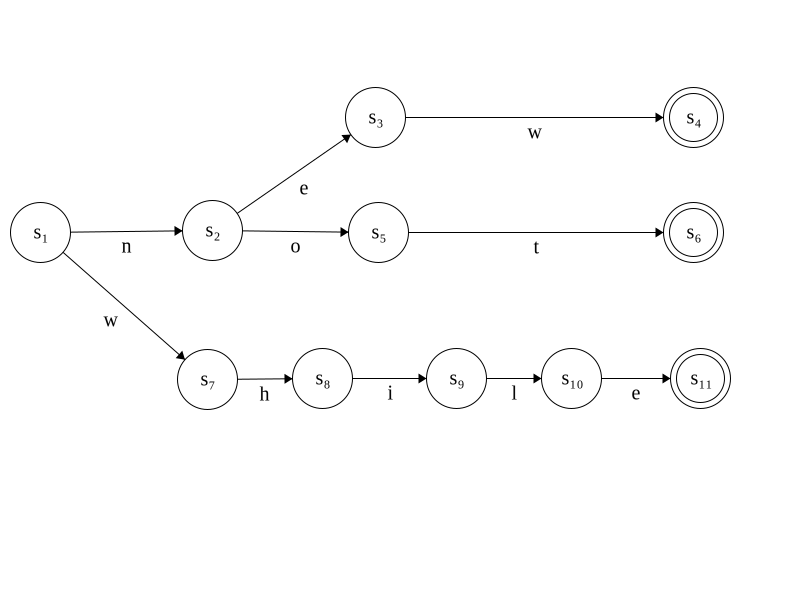
\includegraphics[width=\linewidth]{nnw.png}
\end{center}

{\tiny
\section{Revision History}
07-26-2019: started book\\
07-28-2019: finished ch1, began ch 2\\
}
\\\\
\textit{Think you found a mistake? You probably did. Let me know at \href{mailto:hi@delonshen.com}{hi@delonshen.com} if you want.}
\end{document}
